
\chapter{Pensamento computacional}\label{pensamento-computacional}

A noção de pensamento computacional tem ganhado força desde 2006, ano em que a professora Jeannette Wing, então professora da Universidade Carnegie Mellon, publica um artigo seminal no qual propõe um conjunto de atitudes, ou abordagens, para a resolução de problemas fundamentadas na forma como cientistas da computação e programadores tratam problemas computacionais. 

A definição clássica que muitos autores dão para o conceito é extraído do próprio trabalho da autora que estabelece que pensamento computacional consiste ``numa abordagem para a solução de problemas, desenho de sistemas e entendimento do comportamento humano que se vale de conceitos fundamentais para ciência da computação'' \cite[Tradução nossa]{wing2006}, ou ainda, na capacidade de formular problemas e expressar suas soluções de forma suficientemente clara de tal modo que um computador possa executá-las.

Para o desenvolvimento do tema, faremos a apresentação de três conceitos que consideramos básicos. São eles: os \textbf{algoritmos}, o \textbf{problema computacional} e a \textbf{abstração}. Ao final demonstraremos como esses elementos se articulam para compor o que se entende por pensamento computacional. 

% O desenvolvimento do tema requer adiscussões preliminares. Comecemos com uma apresentação sobre o papel dos algoritmos.

\section{Algoritmos}\label{sec:algoritmo}

Em termos simplificados, um algoritmo nada mais é do que uma solução para um problema que satisfaz as seguintes condições \cite{Piwek2016}:

\begin{itemize}
	\item deve apresentar uma lista sequenciada de passos que levam à solução do problema 
	\item deve ser um processo finito
	\item deve resolver qualquer instância do problema em questão
\end{itemize}

\begin{figure}[!htb]
	\caption{Algoritmo de soma de três números inteiros}
	\begin{center}
	    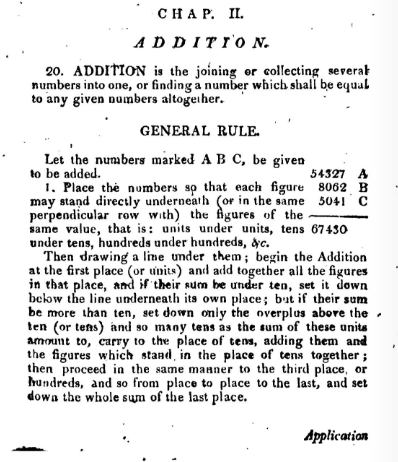
\includegraphics[scale=1]{imagens/algorithm.png}
	\end{center}
	\legend{Fonte: \citeonline{Gough}}
	\label{fig:algoritmo}
\end{figure}

Na figura \ref{fig:algoritmo} lê-se um conjunto de instruções para somar três números inteiros, extraídos do livro \textit{Practical Arithmetick in Four Books} do autor John Gough, publicado pela primeira vez em 1767. Sob o título `General rules', lemos

\begin{citacao}
	Coloque os números de modo que cada algarismo possa ficar diretamente abaixo (ou na mesma linha perpendicular) dos algorismos de mesmo valor, ou seja: unidades em unidades, dezenas em dezenas, centenas em centenas.$[...]$Em seguida, desenhando uma linha abaixo deles; comece a adição no primeiro lugar (ou unidades) e some todas os algorismos naquele lugar, e se a soma delas for menor que dez, coloque-a abaixo da linha abaixo de seu próprio lugar;mas se a soma for superior a dez, estabeleça apenas o excedente acima das dez (ou dezenas) e algumas dezenas, à medida que a soma dessas unidades se eleva, carregue para o local das dezenas, adicionando-as e os algorismos que estão no lugar de dezenas juntos; em seguida, proceda da mesma maneira até o terceiro lugar, ou centenas, e de um lugar para outro até o último, e estabeleça a soma total do último lugar.  
\end{citacao}

Perceba como essas instruções satisfazem as condições elencadas anteriormente: nela vemos um problema (cálculo da soma de três número inteiros) sendo resolvido de forma encadeada ao longo de um processo finito. Nota-se também que os passos acima facultariam a soma de quaisquer outros três números inteiros, atendendo a exigência de ``resolver qualquer instância do problema''. 


\section{Problema Computacional}

A tarefa de definir as instâncias de um problema equivale a determinar para quais perguntas um algoritmo deve oferecer respostas. Em problema de divisão, por exemplo, onde é preciso calcular a razão entre $a$ e $b$, o par $a=1.5$ e $b=9.365$ representa uma delas. Já $a=65.4$ e $b=77$ compõe outra. Numa única sentença podemos resumir que qualquer par de reais, onde $b\neq0$, representa uma instância válida. 

A decisão de usar um computador para a resolução de qualquer problema exige que definamos tais instâncias. Sob o ponto de vista da ciência computação, ao procedermos dessa forma, distinguindo claramente os contornos do problema, definimos um ``problema computacional''.  


A definição clara das instâncias do problema (criação de um problema computacional) e dos passos exatos para sua solução\footnote{Ao tratarmos computacionalmente um problema devemos ser capazes também de distinguir quando e porque, eventualmente, ele não tem solução.} (elaboração de um algoritmo) nos permitirá automatizar a sua execução. 

% E é exatamente nessas duas habilidades que se apoiam o pensamento computacional.

\section{Abstração}

A noção de abstração é outro componente que necessita ser compreendido ao tratarmos do assunto. Nas palavras de \citeonline{wing2006},

\begin{citacao}
A abstração é usada na definição de padrões, generalização de instâncias e parametrização. É usado para deixar um objeto representar muitos. Ele é usado para capturar propriedades essenciais comuns a um conjunto de objetos enquanto oculta distinções irrelevantes entre eles \cite[p.~1. Tradução nossa]{wing2006}
\end{citacao}

Abstrair, como enfatiza o trecho acima, equivale simplesmente a conduzir um processo de generalização, onde incorporamos parte dos detalhes da realidade em um modelo, ao mesmo tempo que descartamos outros. Estabelece-se assim uma relação entre dois níveis: a realidade e sua representação.

\begin{figure}[!htb]
	\caption{Relação entre a realidade e o seu modelo}
	\begin{center}
	    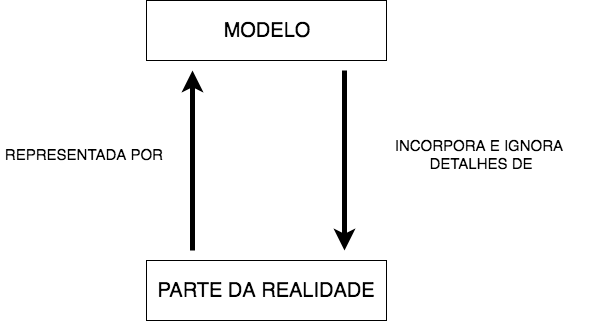
\includegraphics[scale=0.65]{imagens/modelo_e_realidade.png}
	\end{center}
	\legend{Adaptado de \citeonline[]{Piwek2016}}
\end{figure}

A figura \ref{fig:pipe} ilustra essa discussão. Nela vemos a obra ``A Traição das Imagens '' por René Magritte (1898-1967), onde lê-se \textit{``Ceci n'est pas une pipe''} (``Isto não é um cachimbo''). Temos aí provocação que evidencia que um modelo nada mais é do que uma representação, e não a realidade em si.

\begin{figure}[!htb]
	\caption{``A Traição das Imagens'' por René Magritte, 1929}
	\begin{center}
	    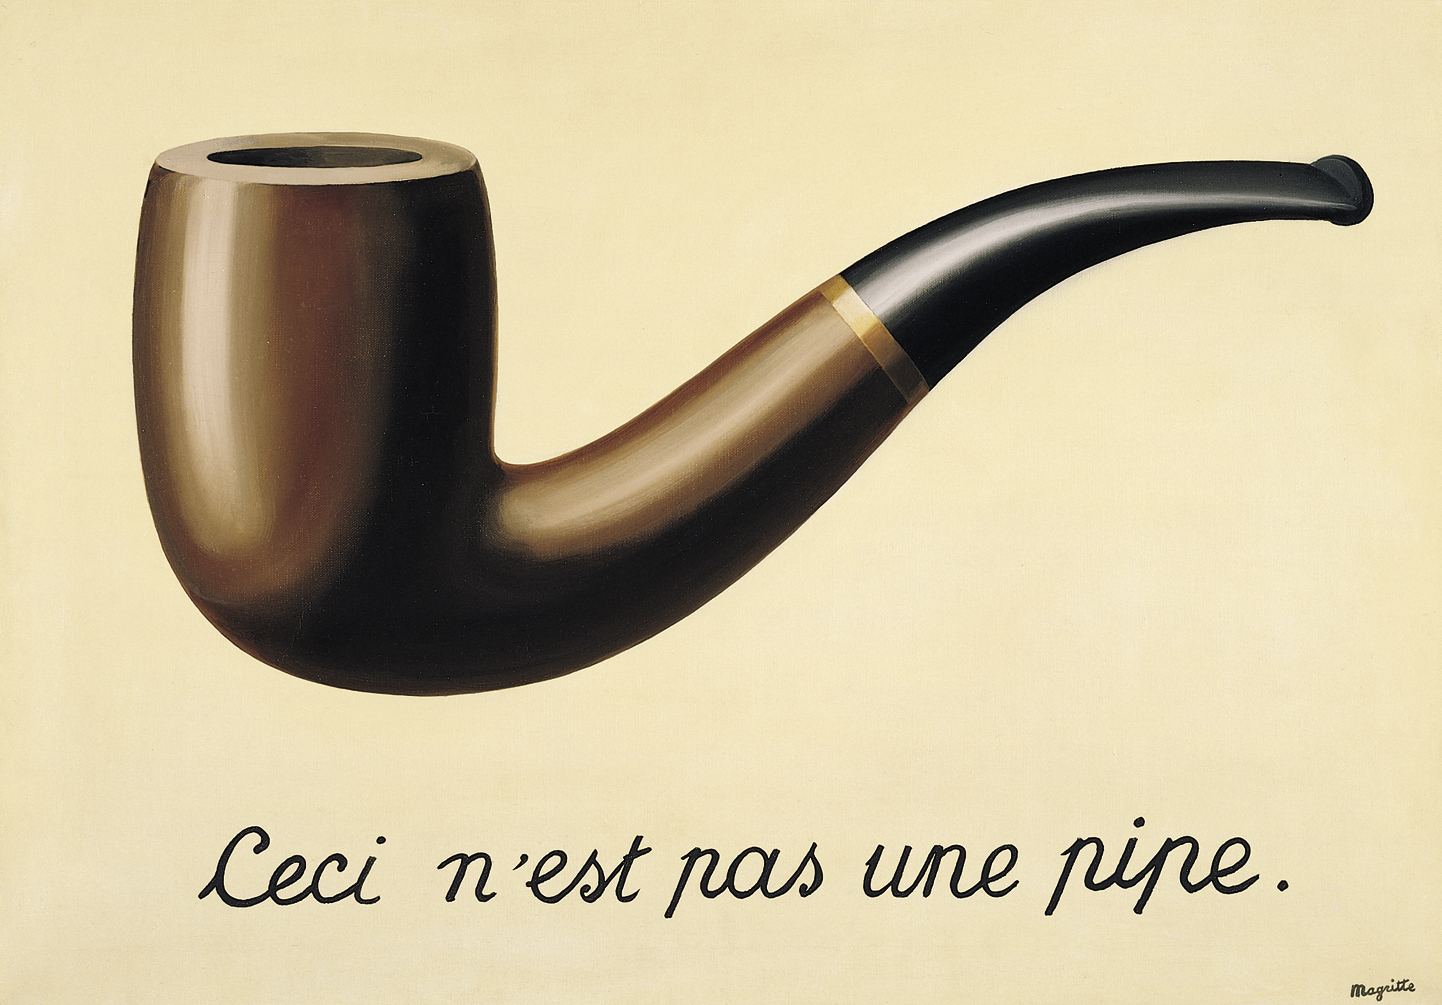
\includegraphics[scale=0.75]{imagens/pipe}
	\end{center}
	\label{fig:pipe}
\end{figure}

O grau de detalhamento do modelo depende das circunstâncias do problema, bem como das necessidades de quem modela. Por exemplo, ao analisarmos a trajetória de lançamento de um foguete, podemos descartar suas dimensões e eliminar possíveis efeitos aerodinâmicos. Essa abordagem é extremamente conveniente para o ensino de primeiras noções de física básica, mas demasiadamente simplória no contexto da condução de um programa aerospacial.

Na figura \ref{fig:cows} temos a ilustração dessa ideia: a mesma ``realidade'' vaca representada por quatro modelos com diferentes graus de detalhes incorporados.

\begin{figure}[!htb]
	\caption{Quatro representações de uma vaca por Theo van Doesburg, 1917--1918}
	\begin{center}
	    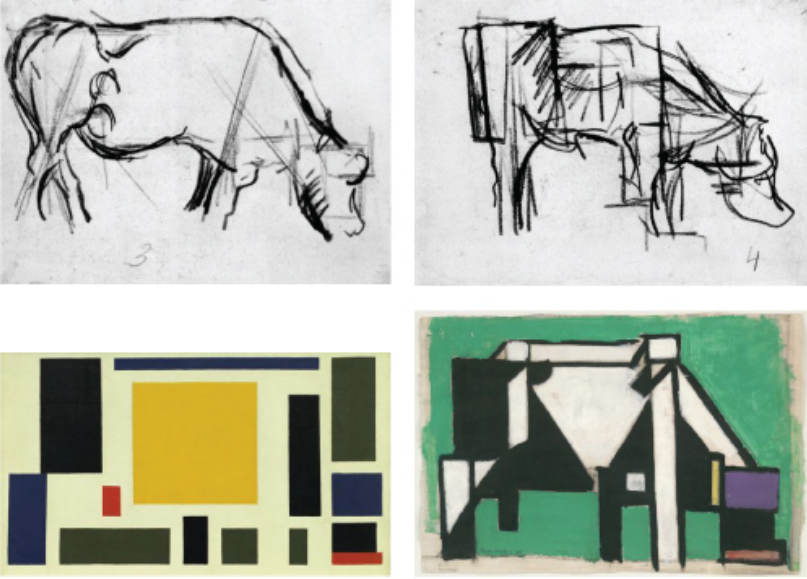
\includegraphics[scale=0.26]{imagens/vacas.png}
	\end{center}
	\legend{Fonte: \citeonline[]{Piwek2016}}
	\label{fig:cows}
\end{figure}

É interessante notar a proximidade do significado para abstração discutido até aqui com aquele proposto pelo filósofo John Locke, segundo o qual formação de uma abstração corresponde a uma transformação durante a qual ``ideias tomadas de seres particulares se tornam representantes gerais de todos do mesmo tipo'' \apud[p.~354. Tradução nossa]{Locke}{Sengupta2013}.

\subsection{Modelos e módulos: duas possibilidade de abstração}

\citeonline[]{Piwek2016} distingue dois tipos de abstrações: a ``abstração como modelo'', onde detalhes da realidade observada são desconsideradas em favor de outras -- o mesmo trabalhado até aqui -- e a ``abstração como encapsulamento'', processo no qual organizamos nosso modelo em módulos ou cápsulas que permitem a composição de sistemas mais complexos. 



Para diferenciarmos esses dois tipos tomemos como ponto de partida o planetário mecânico ilustrado na figura \ref{fig:planetario}. Nele vemos uma simulação do sistema solar, um modelo, que como tal ignora certas aspectos da realidade. Neste caso em específico temos a desconsideração típica de representações astronômicas onde as proporções entre as dimensões dos planetas e a distância relativas entre eles é extremamente grande. A construção de modelos, ignorando e incorporando detalhes, é o que \citeonline{Piwek2016} chama de ``abstração como modelo''. 

\begin{figure}[!htb]
	\caption{Planetário mecânico}\label{fig:planetario}
	\begin{center}
		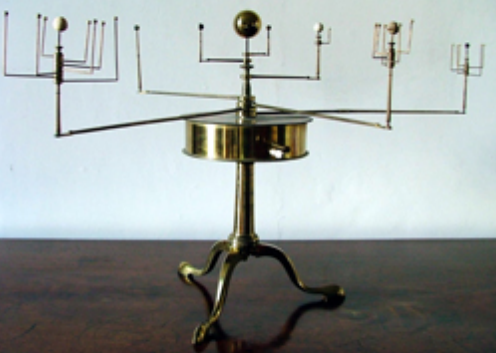
\includegraphics[width=0.50\textwidth]{imagens/planetario}
	\end{center}
	\legend{Fonte: \citeonline{Piwek2016}}
\end{figure}

O mesmo dispositivo incorpora a noção do que o autor chama de ``abstração como encapsulamento''. Na figura \ref{fig:engine} vemos um sistema de rodas dentadas típico do que podemos encontrar no interior de um planetário mecânico. São elas que permitem o movimento das esferas que representam os planetas. A superfície metálica que vemos na figura \ref{fig:planetario} cumpre o papel de interface do modelo ao escondê-las, deixando externamente visível apenas o que é relevante: o movimento de translação e rotação. 

\begin{figure}[!htb]
	\caption{Engrenagem de um planetário mecânico}\label{fig:engine}
	\begin{center}
		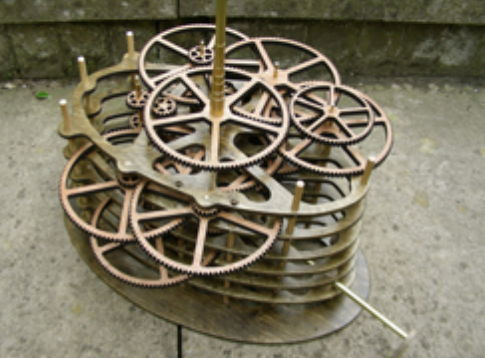
\includegraphics[width=0.50\textwidth]{imagens/engine}
	\end{center}
	\legend{Fonte: \citeonline{Piwek2016}}
\end{figure}

Distingue-se assim a formação de duas camadas durante o processo de encapsulamento: a interface com a qual se pode interagir com o modelo (o invólucro metálico do planetário) e a sua implementação propriamente dita (sistema de engrenagens encerradas pela interface). A figura \ref{fig:encapsulamento} ilustra a relação entre elas.

\begin{figure}[!htb]
	\caption{Interface e implementação -- dois aspectos de um modelo}\label{fig:encapsulamento}
	\begin{center}
		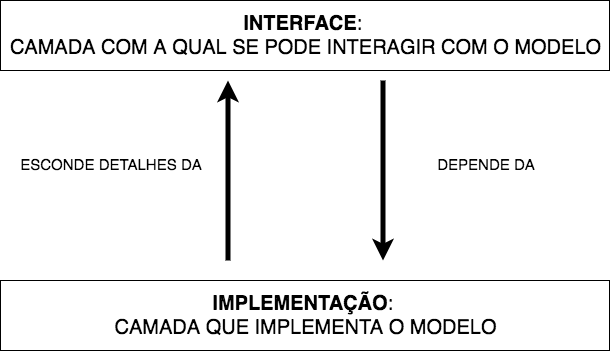
\includegraphics[scale=0.55]{imagens/encapsulamento}
	\end{center}
	\legend{Fonte: \citeonline{Piwek2016}}
\end{figure}

O uso do encapsulamento é essencial na ciência da computação. Nesse contexto, essa estratégia toma forma em funções e estrutura de dados\footnote{Por estrutura de dados nos referimos às diversas possibilidade de organização e relacionamento de dados que uma linguagem oferece. Dentre as mais comuns estão os vetores, as listas, as pilhas...}. Tomemos um exemplo envolvendo funções. Considere a necessidade de calcularmos a seguinte expressão: 

$$\dfrac{(2+3+5 \times 7)}{5}$$

Usando uma linguagem de programação poderíamos reescrever a equação acima do seguinte modo:

\begin{equation*}
	\boxed{razao(\boxed{soma(2,3,\boxed{producto(5,7)})},5)}
\end{equation*}

Perceba a formação de cápsulas. Por exemplo, aos escrevermos $produto(a,b,c \dots)$, estamos modularizando o processo de multiplicação, pois todos os detalhes dessa operação estão invisibilizados atrás de uma interface, cujo nome decidimos chamar como ``produto''. Aplica-se o mesmo raciocínio aos casos das funções $soma(a, b, c...)$ e $razao(a,b)$.

A decomposição do modelo ou sistema pode ganhar tantas unidades quanto se queira, até atingirmos o nível binário (0 e 1s). É exatamente na possibilidade de aplicação recursiva dessa estratégia que a construção de sistemas complexos se tornam viáveis. Esse aspecto é ilustrado na figura \ref{fig:recursividade}.

\begin{figure}[!htb]
	\caption{Decomposição em camadas de um sistema}\label{fig:recursividade}
	\begin{center}
		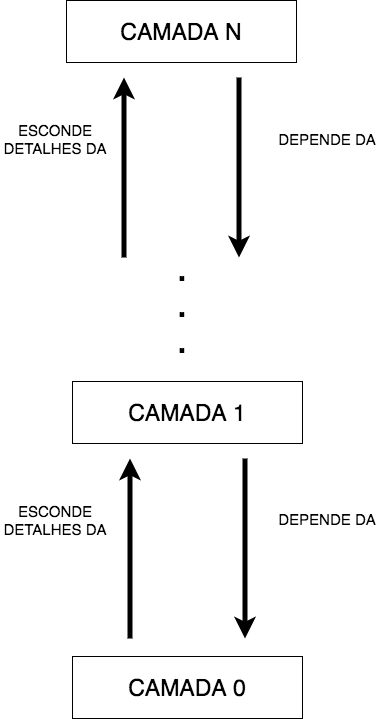
\includegraphics[scale=0.55]{imagens/recursividade}
	\end{center}
	\legend{Fonte: \citeonline{Piwek2016}}
\end{figure}

% De fato, como ressalta \citeonline{Schimidt}, pesquisadores e desenvolvedores programam criand

% Schmidt (2006) aponta que os pesquisadores e desenvolvedores de software normalmente se envolvem na criação de abstrações que os ajudam a programar em termos de seus objetivos de design contextualizados (por exemplo, o problema específico que eles estão resolvendo) em vez do ambiente computacional subjacente (por exemplo, CPU , memória e dispositivos de rede) e protege-os das complexidades desses ambientes.

% O encapsulamento favorece a construção de programas na medida que permite que desenvolvedores expressem seu raciocínio em termos de unidades representativas, ajustando o foco da sua atenção para aspectos do problema que estão resolvendo e permitindo que ignorem as complexidades próprias do ambiente computacional com que estão trabalhando. 

De fato, ao encapsular, programadores buscam expressar-se apenas em termos de unidades representativas. Essa tática permite a eles raciocinar somente em termos do problema que estão resolvendo, e os protege assim das complexidades próprias do ambiente computacional com que estão trabalhando, tal como a necessidade de administrar diretamente o uso da memória, por exemplo. Ao mesmo tempo, por favorecer a organização e a estruturação lógica do código fonte, como vantagem adicional essa abordagem facilita manutenções futuras do sistema. 

Todo o desenvolvimento da computação está assentado na decomposição modular de sistemas. Celulares, computadores, sistemas operacionais, automóveis... Toda e qualquer tecnologia operada por dispositivos eletrônicos. Há exemplos históricos, contudo, onde esse princípio é aplicado apesar de não haver nenhum substrato eletrônico. Na figura \ref{fig:meccano} vemos o primeiro computador programável desenvolvido com o propósito de executar operações matemáticas. Conhecido como Meccano, ele foi proposto por Charles Babbage (1791--1871). Movido a vapor, na imagem temos um exemplar construído em latão e ferro.

\begin{figure}[!htb]
	\caption{Meccano -- Implementação do primeiro computador programável proposto por Charles Babbage }\label{fig:meccano}
	\begin{center}
		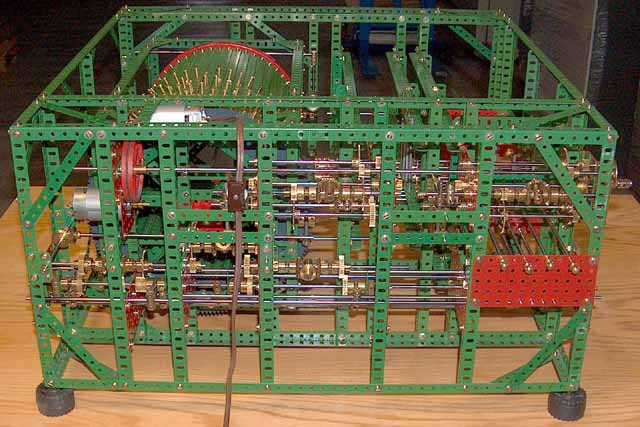
\includegraphics[scale=0.45]{imagens/babbage}
	\end{center}
	\legend{Fonte: \citeonline{Piwek2016}}
\end{figure}

Em suma, a criação de abstrações tanto por modelagem quanto por encapsulamento nos permitem administrar as complexidades do mundo real. Criando modelos, buscamos diminuir os aspectos ruidosos do mundo real em favor de elementos relevantes para a análise do problema, enquanto que ao encapsularmos, como diz \citeonline{Piwek2016}, evitamos ser vitimizados pelos intricados detalhes do ``mundo dos computadores''.

\section{Um apanhado geral}

Até agora apresentamos alguns conceitos sem relacioná-los apropriadamente. Alguns deles:

\begin{itemize}
	\item modelo matemático
	\item problema computacional
	\item algoritmo
	\item abstração como modelo e encapsulamento
\end{itemize}
	
Afinal como esses elementos se articulam em torno do conceito de pensamento computacional, tema-central desse trabalho? Comecemos relacionando os conceitos de modelo matemático e problema computacional.

O propósito da construção de modelos matemáticos se confunde a finalidade da atividade científica: o entendimento e a descrição fenômenos e comportamento de sistemas em função de condições pré-estabelecidas.
 
Na construção de tais modelos, busca-se investigar as regras de interação entre os componentes internos ao sistema investigado e como o ambiente externo influencia essas relações. Fixados alguns parametros, tenta-se entender qual é o papel da variação de alguns outros. Em muitos casos, o objetivo principal desse processo é a formalização dessa descrição em equações matemáticas. Em outros, a validação de descrições já propostas. 

O surgimento do modelo matemático nasce portanto da consolidação das equações que regem o sistema.

Tanto na engenharia quanto nas ciências naturais, o uso de modelos matemáticos tem visado a construção de simulação computacionais. A adoção dessa estratégia favorece o entendimento do comportamento do sistema sob condições limites o que pode evitar, em alguns casos, a ocorrência de tragédias. Ao mesmo tempo, por oferecer um contexto que proporciona o ganho de \textit{insights}, o uso de simulação facilita o desenho de estratégias para otimização de recursos materiais e humanos. 

A figura \ref{fig:modelo_matematico} torna explícita a proximidade entre a construção de um modelo matemático e a resolução de um problema computacional. Como definido na seção \ref{sec:algoritmo}, entende-se como problema computacional um conjunto de perguntas que um computador potencialmente pode responder. A tarefa de resolver o problema computacional, como visto, se resumirá a construção de um algoritmo que leve a cada uma dessas respostas. Igualmente, as equações que compõe um modelo matemático tem como papel tecer uma associação entre um conjunto de parâmetros e uma configuração específica assumida pelo sistema sob observação. Nesse sentido, relações matemáticas e algoritmos cumprem a mesma finalidade.

\begin{figure}[!htb]
	\caption{Elementos de um modelos matemático}\label{fig:modelo_matematico}
	\begin{center}
		\includegraphics[scale=0.50]{imagens/modelo_matematico}
	\end{center}
\end{figure}

Essa forte correlação estrutural é o que tem tornado efetiva a relação entre a ciência da computação e a pesquisa científica. Os elos que integram esses domínios estão visíveis na figura \ref{fig:elos}. 

% O papel do pensamento computacional coordenar os elementos dessa composição.

% \begin{figure}[!htb]
% 	\caption{Visão panorâmica do pensamento computacional}\label{fig:elos}
% 	\begin{center}
% 		\includegraphics[scale=0.25]{imagens/elo}
% 	\end{center}
% \end{figure}
\begin{sidewaysfigure}[!htb]
	\caption{Visão panorâmica do pensamento computacional}\label{fig:elos}
	\begin{center}
		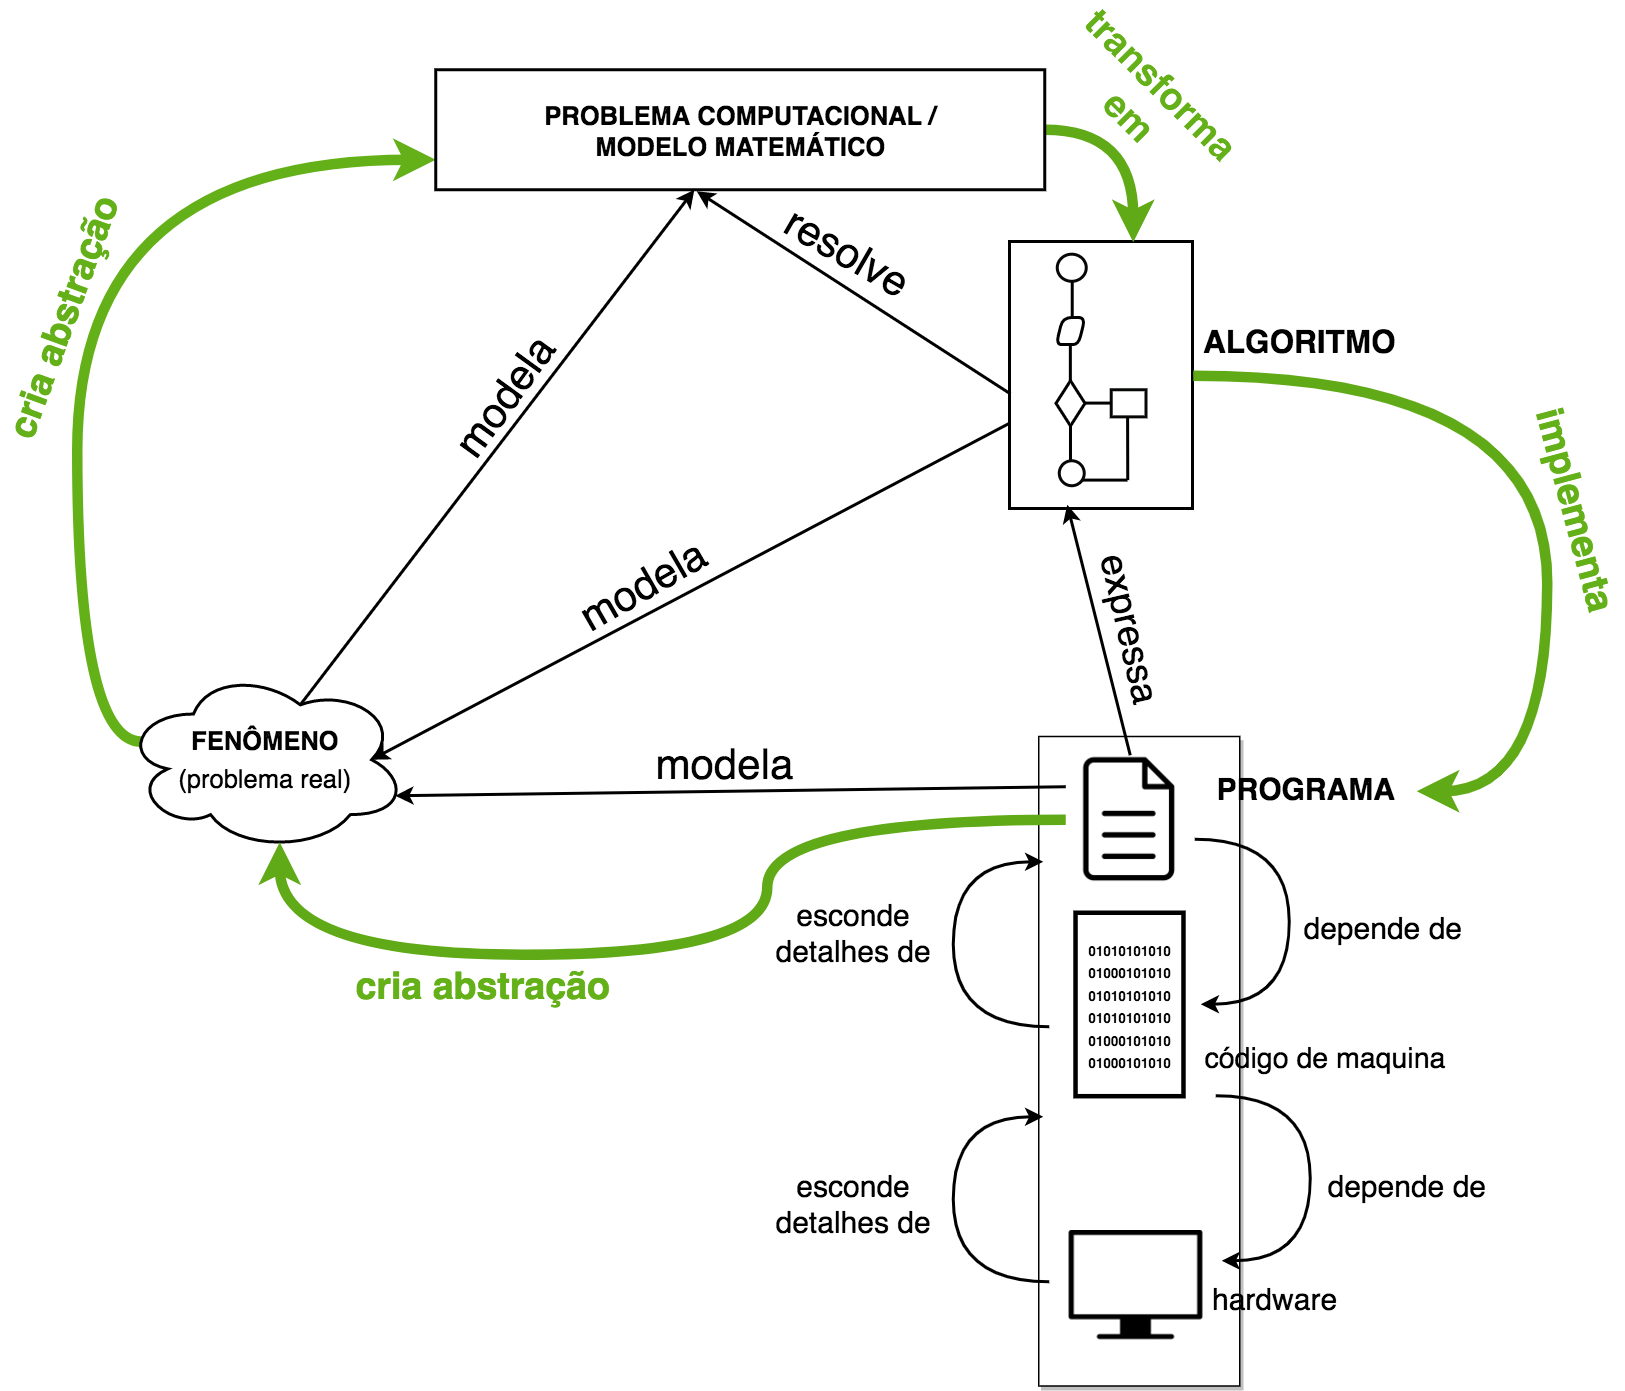
\includegraphics[scale=0.30]{imagens/elos}
	\end{center}
\end{sidewaysfigure}






% De fato, ao permitir a formação de unidades representativas (ou módulos), o encapsulamento permitem ao que os dese

% Além de permitir a construções de modelos (abstração como modelos), a construção de abstrações agrupam outro conceito: `abstração'
% O trecho acima enfatiza a criação de uma abstração como um processo de generalização. Abstrações, desse ponto de vista, são representações generalizadas aplicáveis a diversos contextos ou situações. 

% No contexto da computação científica, o uso de abstrações se dá a partir da construção e do uso de modelos matemáticos. Estabelece-se aí a noção de abstração como modelagem. %mas 

% A necessidade de criação de um modelo nasce normalmente da intenção de se elaborar uma descrição de um sistema ou processo, como no caso das ciências físicas onde se buscam representações para fenômenos da realidade. 

%Essencialmente, ao construirmos um modelo buscamos 

%A tarefa de se construir 